\documentclass{stdlocal}
\begin{document}
\section{Related Work} % (fold)
\label{sec:previous_work}

As marked in the introduction in section~\ref{sec:introduction}, the smoothing of curves on surface meshes is an essential operation for mesh processing and, as a consequence, for many other domain areas, like computer graphics, image-based medicine, and engineering, that rely on such tools \autocite{ji2006,kaplansky2009}.
In most of its applications, initial curves are either provided by means of direct user interaction or by automatic or semiautomatic feature detection algorithms \autocite{zachow2003,lawonn2014}.
The finite precision of the underlying surface mesh together with all the steps included to define an initial curve usually makes resulting lines contain non-smooth artifacts which may violate given constraints or expected properties and therefore degrade its quality \autocite{kaplansky2009,lawonn2014}.
Introducing a smoothing stage into the curve processing pipeline, the mesh segmentation is expected to be of much higher quality which greatly increases its usage for areas like machine learning \autocite{benhabiles2011} or medicine \autocite{zachow2003,alirr2019}.
During the last two decades, there have been multiple successful attempts for constructing algorithms to smooth curves on surfaces \autocite{hofer2004,bischoff2005,lawonn2014,mancinelli2022}.
In this section, a brief overview of their major contributions is given.

\begin{figure}[b]
  \centering
  \begin{subfigure}[t]{0.30\linewidth}
    \centering
    \includegraphics[height=3cm]{images/polthier2006-1.png}
    \caption{\textcite{polthier2006}}
    \label{fig:polthier2006}
  \end{subfigure}
  \begin{subfigure}[t]{0.38\linewidth}
    \centering
    \includegraphics[height=3cm]{images/martinez2005-1.png}
    \caption{\textcite{martinez2005}}
    \label{fig:martinez2005}
  \end{subfigure}
  \begin{subfigure}[t]{0.30\linewidth}
    \centering
    \includegraphics[height=3cm]{images/surazhsky2005-1.png}
    \caption{\textcite{surazhsky2005}}
    \label{fig:surazhsky2005}
  \end{subfigure}
  \caption[Examples of Discrete Geodesics]{%
    \textbf{Examples of Discrete Geodesics}\\
    The images show examples of the different approaches for the generation of geodesics on polyhedral surfaces described by \textcite{polthier2006}, \textcite{martinez2005}, and \textcite{surazhsky2005}.
    All the images have been provided by the authors themselves.
  }
  \label{fig:related-work-geodesics}
\end{figure}

As stated in the previous section~\ref{sec:preliminaries}, a crucial tool for working with curves on two-dimensional manifolds is the ability to find and generate geodesic paths on triangle meshes in the sense of the initial and boundary value problem.
The rigorous mathematical concepts and definitions for the discrete geodesics problems have been elaborated by \textcite{mitchell1987} and \textcite{polthier2006} first published in 1997.
It was marked that the generalization of the concept of geodesics from smooth manifolds to polyhedral surfaces is not unique.
By introducing the notion of discrete geodesic curvature, \textcite{polthier2006} instead fleshed out two main definitions for discrete geodesics on polyhedral surfaces, namely locally shortest geodesics and straightest geodesics.
Both of these concepts coincide on smooth manifolds but differ on polyhedral surfaces resulting in varying solutions to the discrete geodesics problems.
Additionally, \textcite{mitchell1987} built an algorithm to solve the discrete boundary value problem for locally shortest geodesics, that uses a continuous version of the algorithm of \textcite{dijkstra1959} to find the shortest path connecting two given points.
Furthermore, \textcite{polthier2006} provided an iterative algorithm to solve the discrete initial value problem of finding the unique straightest geodesic given a starting point and a direction for which an example can be seen in figure~\ref{fig:polthier2006}.
Hereby, they have proven its correctness and also introduced the notion for parallel translation of vectors along polyhedral surfaces for particle transportation and differential equations.

Based on the results of \textcite{mitchell1987}, \citeauthor{kimmel1998} introduced the so-called fast marching approach (FMM) to efficiently approximate the shortest geodesic connecting two given points, which used the eikonal equation to build propagating fronts and therefore more efficiently generate distance fields \autocite{sethian1996,kimmel1996,kimmel1998}.
\textcite{surazhsky2005} followed with a formulation of exact and approximate algorithms to solve the discrete initial and boundary value problem, which could be evaluated efficiently by the use of such distance fields.
Figure~\ref{fig:surazhsky2005} shows an example of their work.
Extending the idea of distance fields as an intermediate step to the generation of geodesics, \textcite{crane2013} also used the gradient of the heat kernel to reconstruct a distance field by solving the Poisson equation and \textcite{bommes2007} generalized the algorithm of \textcite{surazhsky2005} to not only handle isolated starting points but also general starting polygons on polyhedral surfaces.

\begin{figure}[t]
  \centering
  \begin{subfigure}[b]{0.4\textwidth}
    \centering
    \begin{minipage}{\linewidth}
      \includegraphics[width=\linewidth]{images/sharp2020-2.png} \\
      \includegraphics[width=\linewidth]{images/sharp2020-1.png}
    \end{minipage}
    \caption{\textcite{sharp2020}}
  \end{subfigure}
  \begin{subfigure}[b]{0.58\textwidth}
    \centering
    \includegraphics[width=\linewidth]{images/mancinelli2022-2.png}
    \caption{\textcite{mancinelli2022}}
  \end{subfigure}
  \caption[State-of-the-Art Discrete Geodesic Tracing]{%
    \textbf{State-of-the-Art Discrete Geodesic Tracing}\\
    The left images shows the approaches for the computation and tracing of geodesics on polyhedral surfaces described by \textcite{sharp2020}.
    The right image shows the funnel algorithm scheme of \textcite{mancinelli2022}.
    All the images have been provided by the authors themselves.
  }
  \label{fig:related-work-geodesics-schemes}
\end{figure}

Building on the theory of \textcite{polthier2006}, \textcite{martinez2005} provided an algorithm to solve the discrete boundary value problem for locally shortest geodesics.
Using paths generated by FMM as initial curve for their algorithm, they were able to iteratively improve this curve with an optimization approach making it eventually converge to the exact solution.
An example of their result has been visualized in figure~\ref{fig:martinez2005}.
Improving the idea of \textcite{martinez2005}, \textcite{xin2007} compared various methods to provide an initial path and presented a visibility-based algorithm to determine an exact locally shortest path on polyhedral surfaces after finitely many steps.
Emphasizing this discrete nature of the problem, \textcite{sharp2020} showed that it is possible to find exact geodesic paths for triangle meshes just by intrinsically flipping the edges of the surface mesh and constructed an algorithm, named \textit{FlipOut}, which finds the locally shortest geodesic in the same isotopy class as the initial curve and that is guaranteed to terminate after a finite number of steps.
The algorithm never needs to embed the final, flipped triangulation into the surface again and exhibits real-time performance even for millions of triangles.
One can see an example of the \textit{FlipOut} scheme in figure~\ref{fig:related-work-geodesics-schemes}.
To further improve the computation of locally shortest geodesics in a finite number of steps, \textcite{mancinelli2022} combined the funnel algorithm of \textcite{lee1984} with the ideas of \textcite{xin2007} into a three-stage algorithm that surpasses \textit{FlipOut} due to its superior initial extraction of a triangle strip that results from using an optimized shortest path algorithm on the dual graph of the surface mesh.
For the initial strip, the shortest path algorithm uses an A*-like distance metric and an underlying double ended queue driven by the small-label-first and large-label-last heuristics to avoid the use of a priority queue.
This scheme is also illustrated in figure~\ref{fig:related-work-geodesics-schemes}.
Additional literature covering topics concerned with discrete geodesics on polyhedral surfaces is also well-covered by \textcite{crane2020}.

\begin{figure}[t]
  \centering
  \begin{subfigure}[b]{0.23\linewidth}
    \centering
    \includegraphics[height=2.5cm]{images/morera2008-1.png}
  \end{subfigure}
  \begin{subfigure}[b]{0.23\linewidth}
    \centering
    \includegraphics[height=2.5cm]{images/morera2008-2.png}
  \end{subfigure}
  \begin{subfigure}[b]{0.25\linewidth}
    \centering
    \includegraphics[height=2.5cm]{images/morera2008-3.png}
  \end{subfigure}
  \begin{subfigure}[b]{0.25\linewidth}
    \centering
    \includegraphics[height=2.5cm]{images/morera2008-4.png}
  \end{subfigure}
  \caption[Examples of Subdivision Curves by \textcite{morera2008}]{%
    \textbf{Examples of Subdivision Curves by \textcite{morera2008}}\\
    The images show examples of the curve smoothing approach given by \textcite{morera2008} which used subdivision schemes.
    All images have been provided by the authors themselves.
    Red lines indicate the initially chosen curve and blue lines the resulting smoothed curve.
  }
  \label{fig:morera2008}
\end{figure}

For the actual creation of smooth curves on surfaces, evidence shows that only a few main approaches have emerged.
Presumably, the most intuitive way for a curve smoothing algorithm to work is by using subdivision schemes for polygonal lines, also called corner cutting.
The algorithm thereby subdivides each line segment and positions newly created points in such a way that the resulting curve is smoother than the previous one.
First introduced and used in the planar case by \textcite{chaikin1974} and \textcite{dyn1992}, \textcite{morera2008} generalized the algorithm to polygonal lines on surfaces.
Two examples of this can be seen in figure~\ref{fig:morera2008}.
Unfortunately, the subdivision curve may consist of points located anywhere inside the faces of the underlying mesh.
Hence, its trajectory is not a surface curve in the strong rigorous mathematical sense and might miss essential parts of the mesh.
The objective to construct a robust curve smoothing algorithm dictates that for discrete surfaces all line segments should lie inside a face of the surface.

\begin{figure}[b]
  \centering
  \begin{subfigure}[b]{0.32\linewidth}
    \centering
    \includegraphics[height=3.8cm]{images/lee2002-1.png}
  \end{subfigure}
  \begin{subfigure}[b]{0.32\linewidth}
    \centering
    \includegraphics[height=3.8cm]{images/lee2002-2.png}
  \end{subfigure}
  \begin{subfigure}[b]{0.32\linewidth}
    \centering
    \includegraphics[height=3.8cm]{images/lee2002-3.png}
  \end{subfigure}
  \caption[Examples of Snakes by \textcite{lee2002}]{%
    \textbf{Examples of Snakes by \textcite{lee2002}}\\
    The images show examples of the curve smoothing approach given by \textcite{lee2002} which used a generalization of snakes to detect surface features.
    All images have been provided by the authors themselves.
  }
  \label{fig:lee2002}
\end{figure}


\begin{figure}[t]
  \centering
  \begin{subfigure}[b]{0.39\linewidth}
    \centering
    \includegraphics[height=4cm]{images/hofer2004-1.png}
  \end{subfigure}
  \begin{subfigure}[b]{0.59\linewidth}
    \centering
    \includegraphics[height=4cm]{images/hofer2004-2.png}
  \end{subfigure}
  \caption[Examples of Energy-Minimizing Splines by \textcite{hofer2004}]{%
    \textbf{Examples of Energy-Minimizing Splines by \textcite{hofer2004}}\\
    The images show examples of the design of smooth curves given by \textcite{hofer2004} that used a variational approach to minimize an energy-like functional on the curve.
    All images have been provided by the authors themselves.
  }
  \label{fig:hofer2004}
\end{figure}

The smoothing of curves based on features of the surface mesh for automatic mesh segmentation and cutting has been shown to successfully work by \textcite{jung2004}, \textcite{bischoff2005}, and \textcite{lai2007}.
To classify surface features, \textcite{lai2007} used a feature-sensitive curve smoothing which allowed them to obtain smooth boundaries for mesh features.
Both publications, \textcite{jung2004} and \textcite{bischoff2005}, are building upon the previous work of \textcite{lee2002} and \textcite{lee2004}.
They generalized so-called snakes for two-dimensional manifolds to represent curves on surfaces that are able to find crucial mesh features by providing an initial curve.
Figure~\ref{fig:lee2002} provides some examples of the results achieved by \textcite{lee2002}.
First introduced by \textcite{kass1988} for two-dimensional images, snakes are closed curves that evolve over many iterations to the features of the mesh by minimizing internal and external forces based on curvature, length, and distance to features.
For snakes, the initial shape is completely unimportant.
They are allowed to merge or split, such that a rapid movement towards the features of the mesh is to be expected.
As a direct consequence, feature-based curve smoothing does not allow for arbitrary trajectories and would lead to a curve that may not be assumed to be near the original curve, which makes these algorithms bad candidates for general curve smoothing.

Another approach for representing and generating smooth curves on surfaces is through the use of splines.
\textcite{hofer2004} and \textcite{pottmann2005} determined splines in general manifolds by addressing the design of curves as an optimization problem in the sense of minimizing the curve's overall quadratic energy and using a variational approach to compute a solution.
Their approach is not only applicable to curves on surface meshes but can be used for a much broader variety of cases, including for example the design of rigid body motions.
Some of their results are shown in figure~\ref{fig:hofer2004}.
Alas, for a small number of control points, the resulting curve may still not be assumed to exhibit a close distance to the initially selected curve.
Overcoming this issue would involve adding many more control points and, eventually, a much higher burden for the user who would need to define those points.
According to \textcite{mancinelli2022}, the variational approach to solve the optimization problem for the design of curves is also expected to provide a poor performance for surface meshes that consist of millions of triangles.

\begin{figure}[t]
  \centering
  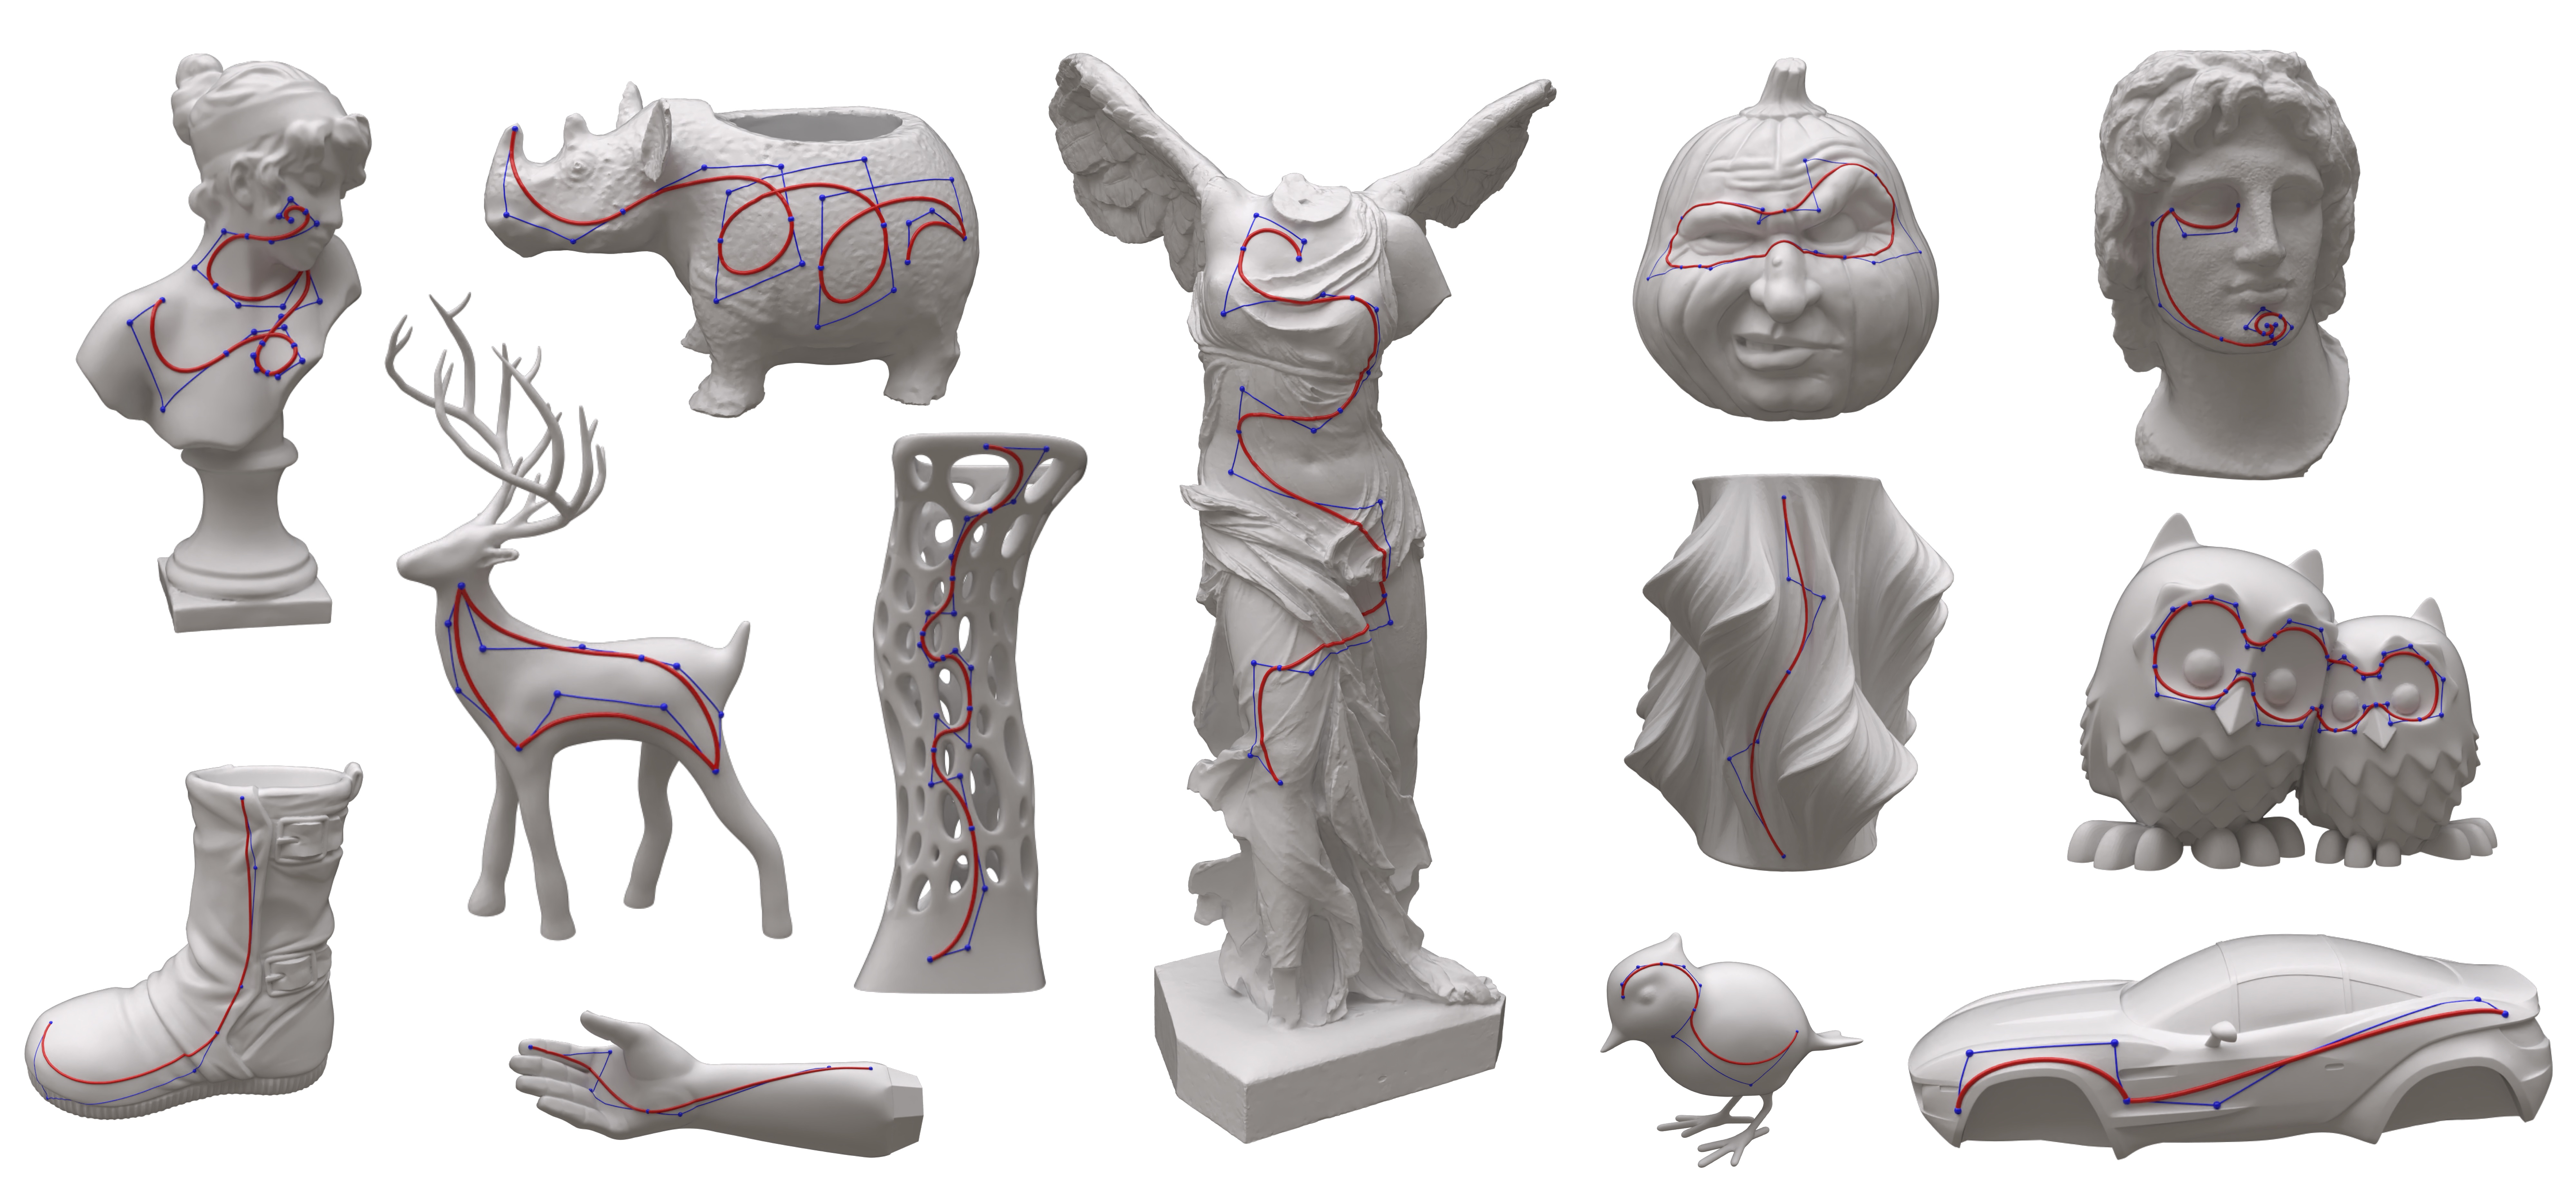
\includegraphics[width=\linewidth]{images/mancinelli2022-1.png}
  \caption[Examples of Bézier Splines by \textcite{mancinelli2022}]{%
    \textbf{Examples of Bézier Splines by \textcite{mancinelli2022}}\\
    The images show examples of the design of smooth curves given by \textcite{mancinelli2022} that used generalized Bézier splines to represent a surface curve.
    Blue lines indicate the initially chosen curve and red lines the resulting spline-based curve.
    All images have been provided by the authors themselves.
  }
  \label{fig:mancinelli2022}
\end{figure}

These results quickly lead to the representation of smooth curves by using generalized Bézier splines.
Two essential contributions are given by \textcite{martinez2007} and \textcite{mancinelli2022}.
They lift the concept of Bézier curves in the two-dimensional Euclidean space to geodesic Bézier splines located in the surface.
The initially chosen curve samples are thereby used as control points to determine the individual shapes of the Bézier splines.
\textcite{mancinelli2022} successfully showed their approach to be superior to other spline alternatives and provided real-time performance when tracing the trajectories of the given splines on the surface for even high-resolution meshes.
In addition, they offer a robust implementation of their algorithm in an open-source C++ framework, named \citetitle{yoctogl} \autocite{agus2019}, that can be found on GitHub \footfullcite{yoctogl}.
The framework is a rather large codebase and a specific documentation for the code responsible for generating, tracing, and controlling Bézier splines could not be found, though.
A whole gallery of examples that has been provided by \textcite{mancinelli2022} can be seen in figure~\ref{fig:mancinelli2022}.
Nevertheless, their approach exhibits similar issues compared to the variational spline approach in that only the use of many control points will make sure that the resulting curve will be near to the initially defined curve.
In this sense, the approach of \textcite{mancinelli2022} does not fit our need by being specialized for vector graphics on surface meshes.

\begin{figure}[t]
  \centering
  \begin{subfigure}[b]{0.29\linewidth}
    \centering
    \includegraphics[height=3.8cm]{images/lawonn2014-1.png}
  \end{subfigure}
  \begin{subfigure}[b]{0.69\linewidth}
    \centering
    \includegraphics[height=3.8cm]{images/lawonn2014-2.png}
  \end{subfigure}
  \caption[Examples of Curve Smoothing by \textcite{lawonn2014}]{%
    \textbf{Examples of Curve Smoothing by \textcite{lawonn2014}}\\
    The images show examples of the curve smoothing algorithm given by \textcite{lawonn2014} that uses a generalization of the algorithm given by \textcite{martinez2005} to fit curvature values.
    Red lines indicate the initially chosen curve and green lines the resulting smoothed curve.
    All images have been provided by the authors themselves.
  }
  \label{fig:lawonn2014}
\end{figure}

Generalizing on the iterative algorithm of \textcite{martinez2005}, \textcite{lawonn2014} created an algorithm for curve smoothing based on curvature values given for each trajectory point.
Each iteration, the algorithm tries to locally fulfill the given curvature constraint, eventually converging to its final smooth curve.
The algorithm guarantees a close distance to the initial curve and can also be used with a simplified user interaction where only one parameter has to be adjusted.
During the process, all iterations adapt to the resolution of the underlying surface mesh and directly provide the curve on the surface without the need of tracing or projection.
The algorithm was shown to be robust against geometric and parametric noise and applied in a medical context, where domain experts evaluated its usability.
\textcite{lawonn2014} proved the convergence of the algorithm and also compared the quality of the generated smoothed curves against the spline-based variational approach without any issue.
Figure~\ref{fig:lawonn2014} shows two examples for this algorithm that visualizes medicine-specific models in the context of mesh cutting.
Furthermore, no surface normals or curvature, that would need to be evaluated first, is needed for the algorithm.
As a result, it may also be formulated for generalized two-dimensional triangular manifolds leaving a wide variety of mesh data structures to choose from \autocite{guibas1985}.
Unfortunately, \textcite{lawonn2014} do not provide any language-specific implementation or performance evaluation.

According to the explanations and descriptions above, for the purpose of this thesis, our design and implementation will mainly focus on the approach given by \textcite{lawonn2014}.
Their algorithm seems to fit our needs in nearly all important aspects.
To solve the potential performance issue and get real-time behavior, a parallelization on the CPU and GPU will be carried out.
We will also strive for an optimized curve initialization and geodesics generation that builds upon the basic building blocks of the approach given by \textcite{mancinelli2022}.

% \autocite{ma2007}
% \autocite{levy2002}
% \autocite{yu2021}
% \autocite{engelke2018}

% section previous_work (end)
\end{document}
